% !Mode:: "TeX::UTF-8"
\documentclass[myposter,portrait]{sciposter}

%% uzitocne package
\usepackage{multicol}
\usepackage{color}
\usepackage{graphicx}

%% znaky s diakritikou
\usepackage[utf8]{inputenc}
\usepackage[T1]{fontenc}
% \usepackage[slovak]{babel} % slovenske delenie slov

%% definicia farieb
\definecolor{mainCol}{rgb}{0.91,0.82,0.74} % farba pozadia posteru
\definecolor{sectionCol}{rgb}{0,0,0} % farba nadpisu
\definecolor{textCol}{rgb}{0.2,0,0} % farba hlavneho textu
\definecolor{BoxCol}{rgb}{1,1,0.8} % farba boxu okolo nadpisov

\def\mysection#1{
{\color{sectionCol}\section*{\sc\bfseries #1}}}

\begin{document}
\setlength{\logowidth}{20cm}
\setlength{\titlewidth}{\textwidth}
\addtolength{\titlewidth}{-\logowidth}
\rightlogo[0.9]{fmfilogo-farebne}
\useleftlogofalse

\color{textCol}

\title{Preparing a Poster for ŠVK is\\
       Really Easy}
\author{Daniel Ševčovič$^1$, Tomáš Vinař$^2$\\
        Supervisor: Tomáš Plachetka$^3$}
\institute{%
$^1$ Katedra aplikovanej matematiky a štatistiky,
FMFI UK, Mlynská Dolina, 842~48~Bratislava\\
$^2$ Katedra aplikovanej informatiky,
FMFI UK, Mlynská Dolina, 842~48~Bratislava\\
$^3$ Katedra informatiky, 
FMFI UK, Mlynská Dolina, 842~48~Bratislava
}
\maketitle

\begin{multicols*}{3}

\mysection{Introduction}
Here we show how easy it is to prepare a poster for ŠVK.
There are some differences in preparing a poster compared to
preparing a paper:

\begin{itemize}
\item use \emph{less text}, since people are not going to stand
      in front of your poster forever and read all your text,
\item use \emph{more figures}, because they quickly draw the
      eye of the reader to the most important points on your poster,
\item use \emph{simple structure} (no numbered theorems, subsections,
      or numbered figures)
\item cite onle \emph{the most important references}
\end{itemize}

\mysection{Sample text}

Let $S=[s_{ij}]$ ($1\leq i,j\leq n$) be a $(0,1,-1)$-matrix
of order $n$. Then $S$ is a {\em sign-nonsingular matrix}
(SNS-matrix) provided that each real matrix with the same
sign pattern as $S$ is nonsingular. 
In this paper we consider the evaluation of integrals of the 
following forms:
\begin{equation}
\int_a^b \left( \sum_i E_i B_{i,k,x}(t) \right)
         \left( \sum_j F_j B_{j,l,y}(t) \right) dt,\label{problem}
\end{equation}
\begin{equation}
\int_a^b f(t) \left( \sum_i E_i B_{i,k,x}(t) \right) dt,\label{problem2}
\end{equation}
where $B_{i,k,x}$ is the $i$th B-spline of order $k$ defined over the
knots $x_i, x_{i+1}, \ldots, x_{i+k}$.

\begin{enumerate}
\item Use Gauss quadrature on each interval.
\item Convert the integral to a linear combination of
      integrals of products of B-splines and provide a recurrence for
      integrating the product of a pair of B-splines.
\item Convert the sums of B-splines to piecewise
      B\'{e}zier format and integrate segment
      by segment using the properties of the Bernstein polynomials.
\item Express the product of a pair of B-splines as a linear combination
      of B-splines.
      Use this to reformulate the integrand as a linear combination
      of B-splines, and integrate term by term.
\item Integrate by parts.
\end{enumerate}

Of these five, only methods 1 and 5 are suitable for our purposes.

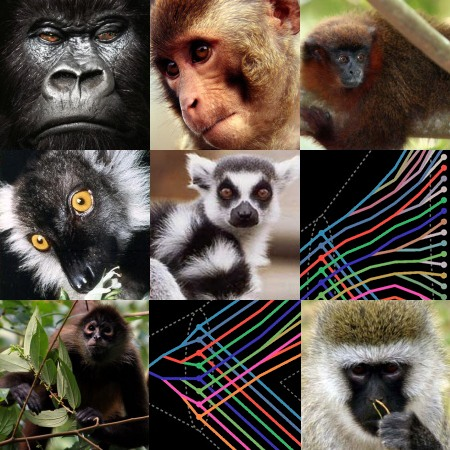
\includegraphics[width=\columnwidth]{allmonkeys}



\mysection{Some displayed equations}
     By introducing the product topology on  $R^{m \times m} \times
R^{n \times n}$  with the induced inner product
\begin{equation}
\langle (A_{1},B_{1}), (A_{2},B_{2})\rangle := \langle A_{1},A_{2}\rangle 
+ \langle B_{1},B_{2}\rangle,\label{eq2.10}
\end{equation}
we calculate the Fr\'{e}chet derivative of  $F$  as follows:
\begin{eqnarray}
 F'(U,V)(H,K) &=& \langle R(U,V),H\Sigma V^{T} + U\Sigma K^{T}\nonumber\\
             && - P(H\Sigma V^{T} + U\Sigma K^{T})\rangle \nonumber \\
         &=& \langle R(U,V),H\Sigma V^{T} + U\Sigma K^{T}\rangle\nonumber \\
&=& \langle R(U,V)V\Sigma^{T},H\rangle + \nonumber\\
  &&    \langle \Sigma^{T}U^{T}R(U,V),K^{T}\rangle.    \label{eq2.11}
\end{eqnarray}

In the middle line of (\ref{eq2.11}) we have used the fact that the range of
$R$ is always perpendicular to the range of $P$.  The gradient $\nabla F$  of
$F$, therefore,  may be interpreted as the
pair of matrices:
\begin{eqnarray}
 \nabla F(U,V) &=& (R(U,V)V\Sigma^{T},R(U,V)^{T}U\Sigma )\nonumber\\
 && \in R^{m \times m} \times R^{n \times n}.   \label{eq2.12}
\end{eqnarray}

Thus, the vector field
\begin{equation}
\frac{d(U,V)}{dt} = -g(U,V) 	\label{eq2.15}
\end{equation}
defines a steepest descent flow on the manifold  ${\cal O} (m) \times
{\cal O} (n)$ for the objective function  $F(U,V)$.

\columnbreak 

\mysection{Numerical experiments} 

We conducted numerical experiments 
in computing inexact Newton steps for discretizations of a  
{\em modified Bratu problem}, given by  
\begin{eqnarray} 
{\displaystyle \Delta w + c e^w + d{ {\partial w}\over{\partial x} } } 
&=&{\displaystyle f \quad {\rm in}\ D, }\nonumber\\[-1.5ex]
\label{bratu} \\[-1.5ex]
{\displaystyle w }&=&{\displaystyle 0 \quad {\rm on}\ \partial D , } \nonumber
\end{eqnarray} 
where $c$ and $d$ are constants. The actual Bratu problem has $d=0$ and  
$f \equiv0$. It provides a simplified model of nonlinear diffusion  
phenomena, e.g., in combustion and semiconductors, and has been 
considered by Glowinski, Keller, and Rheinhardt \cite{GloKR85}, 
as well as by a number of other investigators; see \cite{GloKR85} 
and the references therein. See also problem 3 by Glowinski and  Keller  
and problem 7 by Mittelmann in the collection of nonlinear model 
problems assembled by Mor\'e \cite{More}. The modified problem  
(\ref{bratu}) has been used as a test problem for inexact Newton 
methods by Brown and Saad \cite{Brown-Saad1}.  

\def\gmres{{GMRES}} 
\def\gmresm{{\rm GMRES($m$)}} 

In our experiments, we took $D = [0,1]\times[0,1]$, $f \equiv0$, 
$c=d=10$, and discretized (\ref{bratu}) using the usual second-order 
centered differences over a $100\times100$ mesh of equally 
spaced points in $D$. In \gmres($m$), we took $m=10$ and used fast  
Poisson right preconditioning as before.

\bigskip 
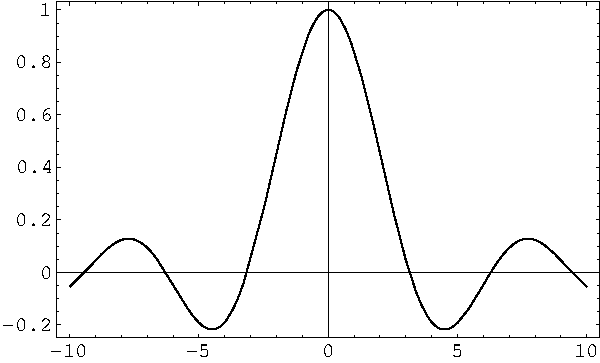
\includegraphics[width=\columnwidth]{fig}
\caption{Graph of the function $\sin(x)/x$.} 
 

%% zoznam literatury
\bibliographystyle{apalike}
\bibliography{references}

\end{multicols*}
\end{document}

